\documentclass[12pt, letterpaper]{article}
\usepackage[titletoc,title]{appendix}
\usepackage{color}
\usepackage{booktabs}
\usepackage[usenames,dvipsnames,svgnames,table]{xcolor}
\definecolor{dark-red}{rgb}{0.75,0.10,0.10}
\definecolor{bluish}{rgb}{0.05,0.05,0.85}
\PassOptionsToPackage{unicode}{hyperref}
\PassOptionsToPackage{naturalnames}{hyperref}
\usepackage[margin=1in]{geometry}
\usepackage[linkcolor=blue,
			colorlinks=true,
			urlcolor=blue,
			pdfstartview={XYZ null null 1.00},
			pdfpagemode=UseNone,
			citecolor={bluish},
			pdftitle={social proof}]{hyperref}

%\newcites{SI}{SI References}
\usepackage{natbib}

\usepackage{float}
\usepackage{placeins}

\usepackage{geometry}  % see geometry.pdf on how to lay out the page. There's lots.
\geometry{letterpaper} % This is 8.5x11 paper. Options are a4paper or a5paper or other...
\usepackage{graphicx}  % Handles inclusion of major graphics formats and allows use of
\usepackage{amsfonts,amssymb,amsbsy}
\usepackage{amsxtra}
\usepackage{verbatim}
%\setcitestyle{round,semicolon,aysep={},yysep={;}}
\usepackage{setspace} % Permits line spacing control. Options are:
%\doublespacing
%\onehalfspace
%\usepackage{sectsty}    % Permits control of section header styles
\usepackage{pdflscape}
\usepackage{fancyhdr}   % Permits header customization. See header section below.
\usepackage{url}        % Correctly formats URLs with the \url{} tag
\usepackage{fullpage}   %1-inch margins
\usepackage{multirow}
\usepackage{verbatim}
\usepackage{rotating}
\setlength{\parindent}{3em}

%\usepackage[T1]{fontenc}
%\usepackage[bitstream-charter]{mathdesign}

\usepackage{chngcntr}
\usepackage{longtable}
\usepackage{adjustbox}
\usepackage{dcolumn}

\usepackage[nameinlink, capitalize, noabbrev]{cleveref}

\def\citeapos#1{\citeauthor{#1}'s (\citeyear{#1})}

\makeatother

\usepackage{footmisc}
\setlength{\footnotesep}{\baselineskip}
\makeatother
\renewcommand{\footnotelayout}{\normalsize \doublespacing}


% Colors
\usepackage{color}

\newcommand{\bch}{\color{blue}\em  }   % begin change
\newcommand{\ying} {\color{orange}\em  }   % begin change
\newcommand{\bgcd} {\color{purple}\em }
\newcommand{\ech}{\color{black}\rm  }    % end change

% Caption
\usepackage{caption}
%\captionsetup[subtable]{font=small,skip=0pt}
\usepackage{subcaption}

% tt font issues
% \renewcommand*{\ttdefault}{qcr}
\renewcommand{\ttdefault}{pcr}


\usepackage{tocloft}


\usepackage{lscape}
\renewcommand{\textfraction}{0}
\renewcommand{\topfraction}{0.95}
\renewcommand{\bottomfraction}{0.95}
\renewcommand{\floatpagefraction}{0.40}
\setcounter{totalnumber}{5}
\makeatletter
\providecommand\phantomcaption{\caption@refstepcounter\@captype}
\makeatother

\usepackage{footmisc}
\renewcommand{\footnotelayout}{\setstretch{2}}

\title{Asymmetry in Cricket: The Effect of Winning the Toss on Winning the Match\thanks{Data and scripts needed to replicate the results are available at: https://github.com/outside-edge/asymmetry/}}

\author{
Apoorva Lal\thanks{Data Scientist, Netflix;  \href{mailto:lal.apoorva@gmail.com}{lal.apoorva@gmail.com }.} \;\;
Derek Willis\thanks{Lecturer in Data and Computational Journalism, University of Maryland;  \href{mailto:dwillis@gmail.com}{dwillis@gmail.com}.}  \;\;
Gaurav Sood\thanks{Independent researcher;  \href{mailto:gsood07@gmail.com}{gsood07@gmail.com}; Corresponding author. Phone: 650 269 7946. Address: 156th Place NE, Redmond, WA, 98052.}\;\;
Avidit Acharya\thanks{Department of Political Science and Graduate School of Business, Stanford University; \href{mailto:avidit@stanford.edu}{avidit@stanford.edu}.}
}
\date{\today}


\begin{document}

\maketitle
\doublespacing

\begin{abstract}

In cricket, which team bats first is determined by a toss. Does the team that wins the toss do better? We find that, on average, the effect of winning the toss on winning the match is essentially nil in international limited-overs daytime matches but substantial (3.3 percentage points) in day/night matches. In Test cricket, the advantage is yet larger (4.9 percentage points). Surprisingly, the effect of winning the toss does not vary substantially across matches between evenly matched and mismatched teams. Lastly, and perhaps most surprisingly, in rain-delayed matches in which the chasing team's total is adjusted by the Duckworth-Lewis formula, we find that the effect of winning the toss is statistically indistinguishable from zero.

\smallskip

\textbf{Key words:} cricket, fairness, randomization

\end{abstract}

\section{Introduction}

In competitive sports, teams fight for every little advantage. Many sports, however, leave some important things to chance. In cricket, a coin toss is used to decide which team bats first. The choice is widely seen as consequential. In many matches, commentators and cricket enthusiasts claim that there is a definite advantage to either bowling or batting first.\footnote{See, for example, the \href{https://www.quora.com/How-much-does-a-toss-matter-to-a-game-of-cricket}{Quora page on ``How much does a toss matter to a game of cricket?''}.} The advantage is also often pointed to by the captains in the pre-toss interview and by the captain of the losing team in the post-match interview.

In this paper, we measure the advantage conferred by winning the toss. To answer the question, we collected data on over 35,000 cricket matches played over 150 years---the largest ever dataset assembled for the question, and more than 50 times larger than used in prominent previous attempts \citep[see,][]{dawson2009bat, de1998winning}. In analyzing these data, we avoid a common but important pitfall that some other studies on the topic fall into. To avoid post-treatment bias \citep[see][]{acharya2015}, unlike \citet{dawson2009bat}, \citet{Saad2015}, etc., we do not condition on post coin-toss decisions. 

We find that winning the toss increases the chances of winning the match by 1.8 percentage points: toss winners prevail 39.2\% of the time and lose 37.4\% of the time; the rest of the matches are drawn or tied. The effect of winning the toss is the largest in Tests, where it is 4.9 percentage points, and the smallest in ODIs and T20s, where it is essentially zero on average. That said, in day/night ODIs and T20s, the effect of winning the toss is 3.3 percentage points.

Contrary to conventional wisdom, the effect of winning the toss does not vary dramatically across continents, though the toss appears less critical on European and African wickets than elsewhere. The effect on Aussie and Kiwi wickets (3 percentage points) is not substantially different from its effect on South Asian wickets (2.8 percentage points) but is higher than on European and African wickets (1.1 and 0 percentage points respectively).

With this, we turn to what teams choose after winning the toss. When pitch and weather conditions are hard to read, many cricket commentators suggest that batting first is the appropriate default choice: get runs on the board and put the opposing team under psychological pressure by having them chase the target. That advice is borne out in the data. Toss winners elect to bat somewhat more often (56.5\% of the time) than they elect to field. However, of the toss winners that elect to bat, only 38.1\% win the match compared to 37.9\% that lose. On the other hand, of the toss winners that opt to field, 40.8\% win the match compared to 36.9\% that lose. This means that 94\% of the 1.8 percentage point effect of winning the toss can be attributed to instances in which the toss-winning team elected to field, and just 6\% of the effect can be attributed to the toss-winning team electing to bat.

Lastly, a caveat about our findings. Our empirical approach estimates the extent to which teams have capitalized on the advantage granted by winning the toss and not the theoretical advantage granted by the toss. The toss may matter a lot in principle, but teams may decide poorly.

The rest of the paper is organized as follows. We start by describing the data. We then analyze if the data are consistent with the toss being random. Next, we present the results. We end with discussing the policy implications.

\section{Data}

We collected data on cricket matches from ESPNCricinfo using a purpose-built library \citep{Willis_python-espncricinfo_A_Python_2022} in June 2020. From the data we collected, we discarded List A matches that were not ODIs or T20s because they are considered a less professional category (with worse data recording). This leaves us with data on all the men's and women's cricket matches in four formats: T20, ODI, Test, and First Class. From this census of the relevant population, we discard matches that were abandoned without the toss being conducted, and a small number of limited-overs (ODI and T20) matches in which the minimum number of overs that must be bowled to establish a result were not bowled. (In ODIs, for example, each side must bat at least 20 overs for a result to be declared.) In all, we dropped 426 matches with ``no result,'' 3 matches that were ``abandoned'' or ``canceled,'' and another three where we have no record for who batted first. The data also suggest little reason to be concerned about biased attrition. The ``no result'' matches, which constitute the overwhelming majority of matches we discard, comprise of matches that were canceled for idiosyncratic reasons, ranging from the \href{https://www.espncricinfo.com/series/shell-tri-series-1991-92-61203/australia-women-vs-england-women-final-66975/full-scorecard}{a team being unable to bat because of the weather} to cancellations because of \href{https://www.espncricinfo.com/series/australia-tour-of-pakistan-1982-83-61392/pakistan-vs-australia-3rd-odi-64196/full-scorecard}{unwanted audience participation}.

Our final sample comprises 35,357 cricket matches across four formats played over 150 years. We report the distribution of matches over time and by type in Figure \ref{fig:timeseries_decomp}. As the figure shows, the number of matches has exploded over the last two decades. This is largely due to the introduction of the enormously popular T20 format of the game; T20 matches constitute over a quarter of all matches played in the last decade.

\section{Is The Toss Random?}

Since our analysis rests on the assumption that the coin toss is random, we start by examining this assumption. Is there any evidence that the coin toss is rigged? For example, does the home side enjoy the rub of the green more often? To study this, we compare the rates at which home teams, teams that won the toss in their last match, and underdogs (defined as the lower-ranked team whenever rankings are available for both teams) win the toss relative to their opponents. We compute the odds of seeing as many successes in the same number of Bernoulli trials with a probability of 0.5. For example, home teams have won 50.8\% of tosses in the 6,377 matches for which we have data. The likelihood of tossing a fair coin 6,377 times and getting as large a percentage of heads is 20.1\%. We find that toss wins are even more balanced for teams that won (lost) the last toss, and for teams that are underdogs and favorites. Table \ref{table: balance} reports these balance results. 

That said, we do see one potential source of concern. We find that teams that share their nationality with at least two of the three umpires of the match win 51.3\% of the tosses in the 4,044 international matches for which we have this data. The likelihood of tossing a fair coin 4,044 times and getting this large a share of heads is only 10\%. This number is certainly low enough to raise some eyebrows. That said, the practice of allowing home-team umpires in international matches ended in 1992, and so these issues are less relevant in recent decades which comprise the bulk of our sample. In addition, a rigged toss in favor of the home team would bias estimates of the advantage of winning the coin toss to the extent that it is correlated with ability. If stronger teams win more tosses, estimates of the advantage of the coin toss would be inflated upwards. And vice versa, if otherwise. Given that home teams win more matches and are seen as stronger, it is possible that the results are biased upwards. For now, we proceed as if the toss was random.

\section{The Effect of Winning the Toss on the Probability of Winning}

To estimate the advantage of winning the toss, we run regressions on a team $\times$ match-level dataset. Let $i$ index teams, and $j$ index matches. $Y_{ij}$ is a dummy for team $i$ winning match $j$, and takes a value of $0.5$ for draws. $Z_{ij}$ is a dummy for team $i$ winning the toss in match $j$. For the main specifications of interest, we estimate regression equations of the form

\begin{equation}\label{eqn:reduced_form}
Y_{ij} = \alpha_0 + \tau Z_{ij} + \gamma_i + \delta_t + \psi_k + \varepsilon_{ij}
\end{equation}

which include fixed effects for teams $\gamma_i$, time $\delta_t$, and match-type $\psi_k$. We cluster the standard errors at the match level.

We report results in Table \ref{table:reduced_form}. The first column gives the baseline estimate of the toss effect. We progressively add team, match-type, and time period fixed effects in columns 2, 3, and 4, and find that the results are remarkably stable. The baseline estimate of 1.8 percentage points reflects the fact that toss winners win 39.2\% of the time and lose 37.4\% of the time; the remaining matches are drawn. The estimated effect shuffles to 1.7 percentage points when we add various fixed effects.

We next examine the effect of the toss across various subgroups. We report the estimates graphically in Figures \ref{fig:rf_het_TE} - \ref{fig:rf_het_TE3} with point estimates and sample sizes as annotations. We summarize the results below:
\begin{itemize}
\item \textbf{Format.} Toss effects are most pronounced in Test matches followed by first-class matches, and are statistically indistinguishable from zero in ODIs and T20s. The effect of the toss on winning a Test match is 4.7 percentage points and 2.3 percentage points in first-class matches. These results support the conventional wisdom among lay cricket followers that the toss grants the greatest advantage in multi-day affairs. Pitches invariably deteriorate over the course of these matches, and the fourth innings of a Test match is often the most challenging time to bat. The pitch deteriorates far less over the course of a day or in the case of T20s, a few hours. Our null results for limited over matches also extend \citet{de1998winning}, who, based on analysis of data from 427 international one-day matches conclude that ``winning the toss at the outset of a match provides no competitive advantage.''

\item \textbf{International vs.~Domestic matches.} Toss effects are virtually the same for international and domestic matches (point estimates are 1.7 percentage points in the former and 1.9 percentage points in the latter). 

\item \textbf{Effects over time.} Toss effects appear to have declined over time from a high of 9.9 percentage points in the second half of the 19th century to 1.4 percentage points in the last decade. This trend may be a result of a changing composition of matches so we also looked at trends within formats. T20s have not been played long enough for us to draw any conclusions about how toss effects have changed over time. But in the other formats, except for Test cricket, where there has been an uptick in the last decade, we find a similar pattern as above. The potential reasons for the decline are numerous. For example, cricketers may have become fitter, and more able to play for long periods without tiring as much as they once did, reducing the impact of the order in which they batted. Pitches may have become more resilient to wear than they once were. Teams may have become better informed about how to play more effectively whether they bat first or second, etc.

\item \textbf{Relative strength.} We expect the toss to be less important in matches where one team is clearly stronger than the other. We expect the stronger team to win, whether it bats first or second. To test this hypothesis, we use team ranking data published by cricket's official governing body, the International Cricket Council (ICC). The median difference between teams is 17 points. We use that as an approximate splitting point, splitting the matches into teams where the gap in the ICC ratings of the two teams is less than 15 points and where it is more. In this case, we believe the standard errors are too large for us to draw substantively meaningful conclusions. 

\item \textbf{Continents.} Toss effects vary somewhat across continents, hovering around 2.5 percentage points for matches played in Asia, Oceania, and the Americas (though the estimates for the Americas are noisier in part due to the smaller number of matches played there). In Europe (effectively England) the toss effect is only 1.1 percentage points (though we cannot rule out a null effect), and in Africa, it is essentially zero. 

\item \textbf{Day/Night matches.} It is often claimed that the toss is more crucial in day-and-night matches. Part of the claim rests on the theory that batting is easier when there is dew, which generally comes in the evening. Another popular theory is that the ball used for day/night limited overs cricket is harder to see at night. We do have the data to adjudicate between the theories but have data that shows that the toss is more consequential in day/night limited over games. In the limited overs formats where day/night matches take place (ODIs and T20s), the advantage of winning the toss is 3.3 percentage points, compared to 0 for limited overs matches during the day. 

\item \textbf{Seasonality.} Weather is thought to have a large impact on the playing conditions in cricket. Cool overcast weather, for example, is thought to aid swing bowling, especially on English pitches. More generally, the advantage of winning the toss likely varies by weather. Although we do not have data on the weather, we can proxy it with seasons. In particular, students of the game suspect that the advantage of winning the toss in the early English season is especially significant. There is some evidence of a seasonal pattern for matches played in England, with the advantage of winning the toss growing over the summer, though the trend is weak and broken in the month of July.

\item \textbf{Rain delays.} Finally, we look at the differential effects of winning the toss in ODI matches that were rain-delayed, causing the number of overs bowled in the second innings to be adjusted down. We examine the subset of matches where rain delays result in revised targets computed using the \citet{duckworth1998} method. This method has been the subject of much controversy, with many cricket fans suggesting that it is rigged against the chasing team. To our surprise, we find no evidence that toss winners are able to exploit the prediction of rain delays to their advantage. If anything, we see that the toss-winners have a 2.4 percentage points \emph{disadvantage} in matches subject to the Duckworth-Lewis adjustment, though this point estimate is statistically indistinguishable from zero.\footnote{Toss-winners won 160 out of 333 ODIs with the Duckworth-Lewis adjustment (i.e.~48\%) and 3,085 out of 6,187 ODIs without the Duckworth-Lewis adjustment (49.9\%).} 

\end{itemize}

\section{Batting Vs. Fielding First}

56.5\% of teams that won the toss elected to bat. This is not surprising given the conventional wisdom is that when you are not sure about whether it is advantageous to bat or field first, bat first. The first column of Table \ref{table:iv_table} shows that 49.2\% of teams that batted first won the match, while 50.8\% of teams that fielded first won. The second column shows that among teams that won the toss and batted first the ``win-loss differential'' is small: these teams won only 0.2 percentage points more frequently than they lost, winning 38.1\% of matches and losing 37.9\% of matches, as reported in the introduction. This win-loss differential is smaller than it is for teams that won the toss and elected to field. The third column of the table shows that these teams won 3.9 percentage points more frequently than they lost: they won 40.8\% of their matches and lost 36.9\% of them. Combining this information with the fact that 56.5\% of teams that won the toss elected to bat (and only 43.5\% elected to field, as implied by the fourth column of the table), we learn that 94\% ($= .435 \times .039/.018$) of the 1.8 percentage point advantage to winning the toss that we reported in the previous section can be attributed to the success of toss-winning teams that elected to field. To further understand what explains the preference to bat or bowl first, we see how winning the toss affects the choice in various subsets:

\begin{itemize}
\item \textbf{Format.} Teams prefer batting first in longer match formats. In Test matches 72.8\% of teams that win the toss bat first, whereas in T20s and ODIs this share is only about 52.9\%. In first-class matches it is 56.9\%. 

\item \textbf{International vs. Domestic matches.} We see no big differences in the propensity to bat first across international versus domestic matches.

\item \textbf{Effects over time.} Historically, toss-winning teams tilted heavily in favor of batting first, but this declined over the course of the 20th century, and now they show no preference (on average) to bat first. Even in test matches, toss-winning teams tend to be tilting less toward batting first than they once did. Pre-1950, more than 90\% of the teams that won the toss elected to bat, whereas in the last two decades that number has been closer to two-thirds. Perhaps players have gotten fitter and are willing to trade off expecting to have to bat on the final day of the match in favor of taking advantage of playing conditions that are favorable to fielding first. As for ODIs, teams interestingly heavily preferred fielding first in the early decades of the format, but in the last thirty years, they have tilted more towards batting first, with just over half of the toss-winning teams electing to bat.

\item \textbf{Relative strength.} We see no notable differences in the toss-winning captain's choice to bat first across matches that are lopsided and those in which the teams are more evenly matched. This is especially true in Tests but also appears to be true in ODIs, though a slightly larger share of toss-winning teams elect to bat in matches that are lopsided (54.6\%) in comparison to ones that are less lopsided (51.9\%).

\item \textbf{Continents.} Toss-winning captains show a preference to bat first in matches played in Oceania and Europe, more so than on other pitches. For example, in Europe (mainly England) $64.9\%$ of toss-winning teams elect to bat, and in Oceania, this number is $59.9\%$. By contrast, on Asian wickets, it is only $50.1\%$.

\item \textbf{Day/Night matches.} The ball being harder to see at night afflicts both batting and fielding. But the difficulty for batsmen is probably greater than it is for fielders. Indeed, within the shorter formats, the variation between day matches and day/night matches is greatest when it comes to the choice to bat first. In day/night matches, $59\%$ of toss-winning teams elect to bat first, whereas in day matches just about half of them do.

\item \textbf{Seasonality.} The preference to bat first in England follows a broadly similar trend to the toss effect over the course of the year-- rising steadily over the summer and dropping in September. At its peak in August, top-winning captains choose to bat first $71.9\%$ of the time. At its lowest in April, the teams that win the toss choose to bat $57.4\%$ of the time.

\item \textbf{Rain delays.} Remarkably, there is an overall preference to field first in matches that ended up using the Duckworth-Lewis adjustment: only $43.5\%$ of toss-winning teams elected to bat in these matches. If captains have the ability to predict rain (and other) delays, they seem to prefer to bat fewer overs and chase the adjusted target.

\end{itemize}

\subsection{The Difficulty in Estimating the Advantage to Electing to Bat/Field First}

Despite reporting the `reduced form' and `first stage' effects of the toss, we cannot interpret the ratio of these effects as the causal effect of batting first. If we used the toss as an instrument for batting first, say, we could at best hope to estimate the local average treatment effect (LATE) of electing to bat on winning the match \citep{angrist1996identification}. This is because in our setting treatment effects likely vary across groups: some teams in some circumstances will be better able to capitalize on batting first.  

However, even the conditions under which the LATE is identified are not satisfied in our setting. To see why, first note that our setting has two-sided noncompliance: there are teams that win the toss that bat first and those that lose the toss that bat first as well. Then, recall that under two-sided noncompliance, the LATE is identified under a monotonicity assumption that rules out defiers. However, defiers are likely to be present in our setting: they correspond to dyads of opposing teams that walk onto the pitch intending to field first if they win the toss. In such a setting, the team that wins the toss will choose to field first and the team that loses the toss will be compelled to bat first. If these defiers are present, which they likely are, the monotonicity assumption does not hold, so we cannot assert that the IV estimates are giving us the LATE.

We make these points more concrete. Recall that we saw that 56.5\% of teams that won the toss elect to bat, which is 6.5 percentage points more than what you would expect if the toss had no effect on the batting/fielding decision. In addition, the reduced form estimated effect of winning the toss on winning the match was 1.8 percentage points, implying that toss winners win an excess of 0.9 percent of matches over parity. The instrumented effect of batting first would then be estimated as 0.9/6.5 = 13.9 percentage points.\footnote{Since the choice to field first is the perfectly colinear inverse of the choice to bat first, flipping the sign of this number gives the estimated instrumented effect of electing to field first.} Can we interpret this as the average rate at which the complier teams that won the toss and elected to bat generated the excess wins? No, because these excess wins could have been generated by the defiers making good decisions to field. Since we saw that teams that win the toss and elect to field first have a higher win-loss differential than those that elect to bat first, it would be irresponsible to rule out this possibility. Consequently, it is unlikely the LATE can be identified in our setting.

\section{Policy Proposals}

The data suggest that in certain kinds of cricket matches, e.g., Day/Night matches and Tests, the team that wins the toss wins the match significantly more often. However, from one perspective, this is not a problem. Given that the toss is random, no team has an advantage in expectation. But this view has at least two problems. First, for the advantage to average out, we need a series of games. This isn't always the case, especially in big tournaments. Second, in each match, the toss grants an advantage to one of the teams before the match starts. This makes matches less interesting when the decision of who bats first is pivotal to the outcome. Furthermore, elsewhere, the rules of cricket already try to correct the asymmetry between teams that bat first and those that bat second. In rain-delayed one-day matches, the Duckworth-Lewis formula is used to set a new target for the chasing team. The argument that no side was advantaged \emph{ex-ante} could have been used to justify not doing any correction in such rain-delayed matches, and simply declaring that the team that batted first won the match because the chasing team was unable to reach its target. But the designers of one-day cricket were clearly unwilling to allow the bad luck of weather to have this much influence on the game. If addressing the misfortunes of weather is important, it may also be important to address the misfortune of losing the toss.

For those who take this latter view, there are a variety of policy levers. For instance, to address the large advantage in day/night ODIs and T20s, one way institute a policy of not holding day/night matches. Or, as some English counties have done, the right to choose whether to bat or bowl first can be given to the visiting team. Or, we may want to build wickets that do not deteriorate appreciably. Or, institute a baseball-like innings system where short innings are interspersed so that no one team benefits from the conditions. All of these solutions likely have deleterious side effects. For instance, making pitches less prone to deterioration means that certain kinds of bowling (spin) will have less of an impact robbing the game of an interesting aspect. A better solution may be to auction off the ability to choose whether to bat or bowl first \citep{sood2021}. Ask teams to use their knowledge and experience to price the value of getting to pick whether to bowl or bat first. We propose giving teams time to inspect the playing surface and then asking the teams to place bids for how many runs should be added to the other team's total. The team with the highest bid wins the right to choose whether to bowl or bat. (If the bids are tied, which suggests that teams price the ability to choose the same, an actual coin toss can be used to decide which team chooses and the runs would be added to the other team's score.) Such ways of resolving who has the right to make the choice to bat or field first could make games more competitive, and thus more enjoyable to many viewers. 

\section*{Acknowledgements}
This paper incorporates some of the text and results from Sood \& Willis's (2016) working paper \href{https://arxiv.org/abs/1605.08753}{Fairly Random: The Impact of Winning the Toss on the Probability of Winning} \citep{sood2016fairly}. The authors thank Matt Blackwell, Andrew Gelman, Donald Green, Jens Hainmueller, and Daniel Stone for their comments.
\newpage
\bibliographystyle{agsm}
\bibliography{biblio.bib}

\clearpage

\begin{table}[htb!]\centering
\caption{Is the toss random? \label{table: balance}}
\begin{tabular}{llll}
\hline
 & Toss Wins & Matches & $p$ value\\ \hline
Home team & 3240 & 6377 & 0.201\\
Last toss winners & 17189 & 34283 & 0.611\\
Underdog & 2001 & 4054 & 0.423\\
Home Umpire &  2075	& 4044	& 0.098 \\ \hline
\end{tabular}
\end{table}

\clearpage

\begin{table}[htb!]
\centering
\caption{The effect of winning the toss on the probability of winning.}

\begin{tabular}{@{\extracolsep{5pt}}lcccc} 
\\[-1.8ex]\hline \\[-1.8ex] 
\\[-1.8ex] & (1) & (2) & (3) & (4)\\ 
\hline \\[-1.8ex] 
 Win Toss & 0.018$^{***}$ & 0.017$^{***}$ & 0.017$^{***}$ & 0.017$^{***}$ \\ 
  & (0.005) & (0.005) & (0.005) & (0.004) \\ 
  Constant & 0.491$^{***}$ &  &  &  \\ 
  & (0.002) &  &  &  \\ 
 Team FE &  & $\checkmark$ & $\checkmark$ & $\checkmark$ \\ 
Match-Type FE &  &  & $\checkmark$ & $\checkmark$ \\ 
Time FE &  &  &  & $\checkmark$ \\ 
\hline &  &  &  &  \\ 
Number of Matches & 35357 & 35357 & 35357 & 35357 \\ 
\hline \\[-1.8ex] 
\end{tabular} 

\label{table:reduced_form}
\end{table}

\clearpage

\begin{table}[htb!]
\scriptsize
\centering
\caption{The choice to bat first and the probability of winning.}

\begin{tabular}{@{\extracolsep{5pt}}lccccccc} 
\\[-1.8ex]\hline \\[-1.8ex] 
 & \multicolumn{3}{c}{OLS} & First-Stage & \multicolumn{3}{c}{IV} \\ 
\\[-1.8ex] & (1) & (2) & (3) & (4) & (5) & (6) & (7)\\ 
\hline \\[-1.8ex] 
 Bat First & $-$0.016$^{***}$ & 0.002 & $-$0.039$^{***}$ &  &  &  &  \\ 
  & (0.005) & (0.006) & (0.007) &  &  &  &  \\ 
  Win Toss &  &  &  & 0.130$^{***}$ &  &  &  \\ 
  &  &  &  & (0.005) &  &  &  \\ 
  Bat First (IV) &  &  &  &  & 0.139$^{***}$ & 0.134$^{***}$ & 0.134$^{***}$ \\ 
  &  &  &  &  & (0.036) & (0.036) & (0.036) \\ 
  Constant & 0.508$^{***}$ & 0.499$^{***}$ & 0.519$^{***}$ & 0.435$^{***}$ & 0.430$^{***}$ &  &  \\ 
  & (0.002) & (0.003) & (0.004) & (0.003) & (0.018) &  &  \\ 
 Sample & All & TW bats & TW fields & All & All & All & All \\ 
FS F-Stat &  &  &  &  &  & 604.71 & 579.95 \\ 
Team FE &  &  &  &  &  & $\checkmark$ & $\checkmark$ \\ 
Match-Type FE &  &  &  &  &  & $\checkmark$ & $\checkmark$ \\ 
Decade FE &  &  &  &  &  &  & $\checkmark$ \\ 
\hline &  &  &  &  &  &  &  \\ 
Number of Matches & 35357 & 19971 & 15386 & 35357 & 35357 & 35357 & 35357 \\ 
\hline \\[-1.8ex] 
\end{tabular} 

\label{table:iv_table}
\end{table}

\clearpage

\begin{figure}[tbh]
  \centering
  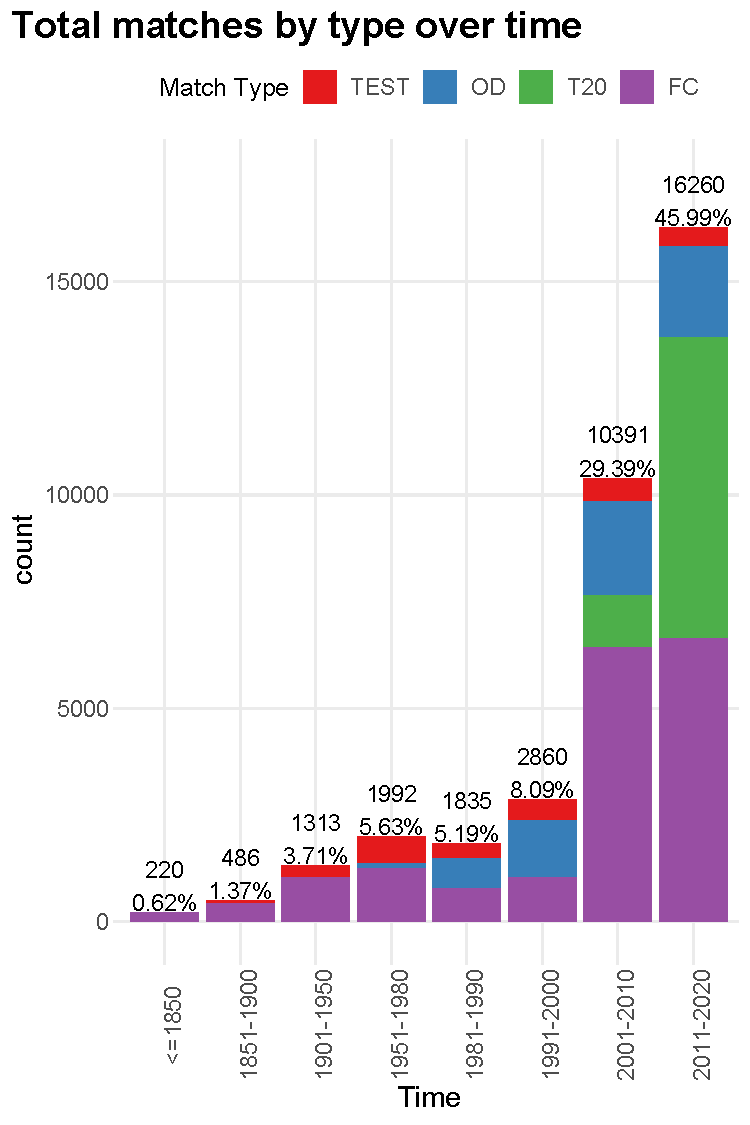
\includegraphics[width=0.6\textwidth,keepaspectratio]{output/matchcounts.pdf}
  \caption{Number of matches by format over time.}
  \label{fig:timeseries_decomp}
\end{figure}

\clearpage
    
\begin{figure}[b]
  \centering
  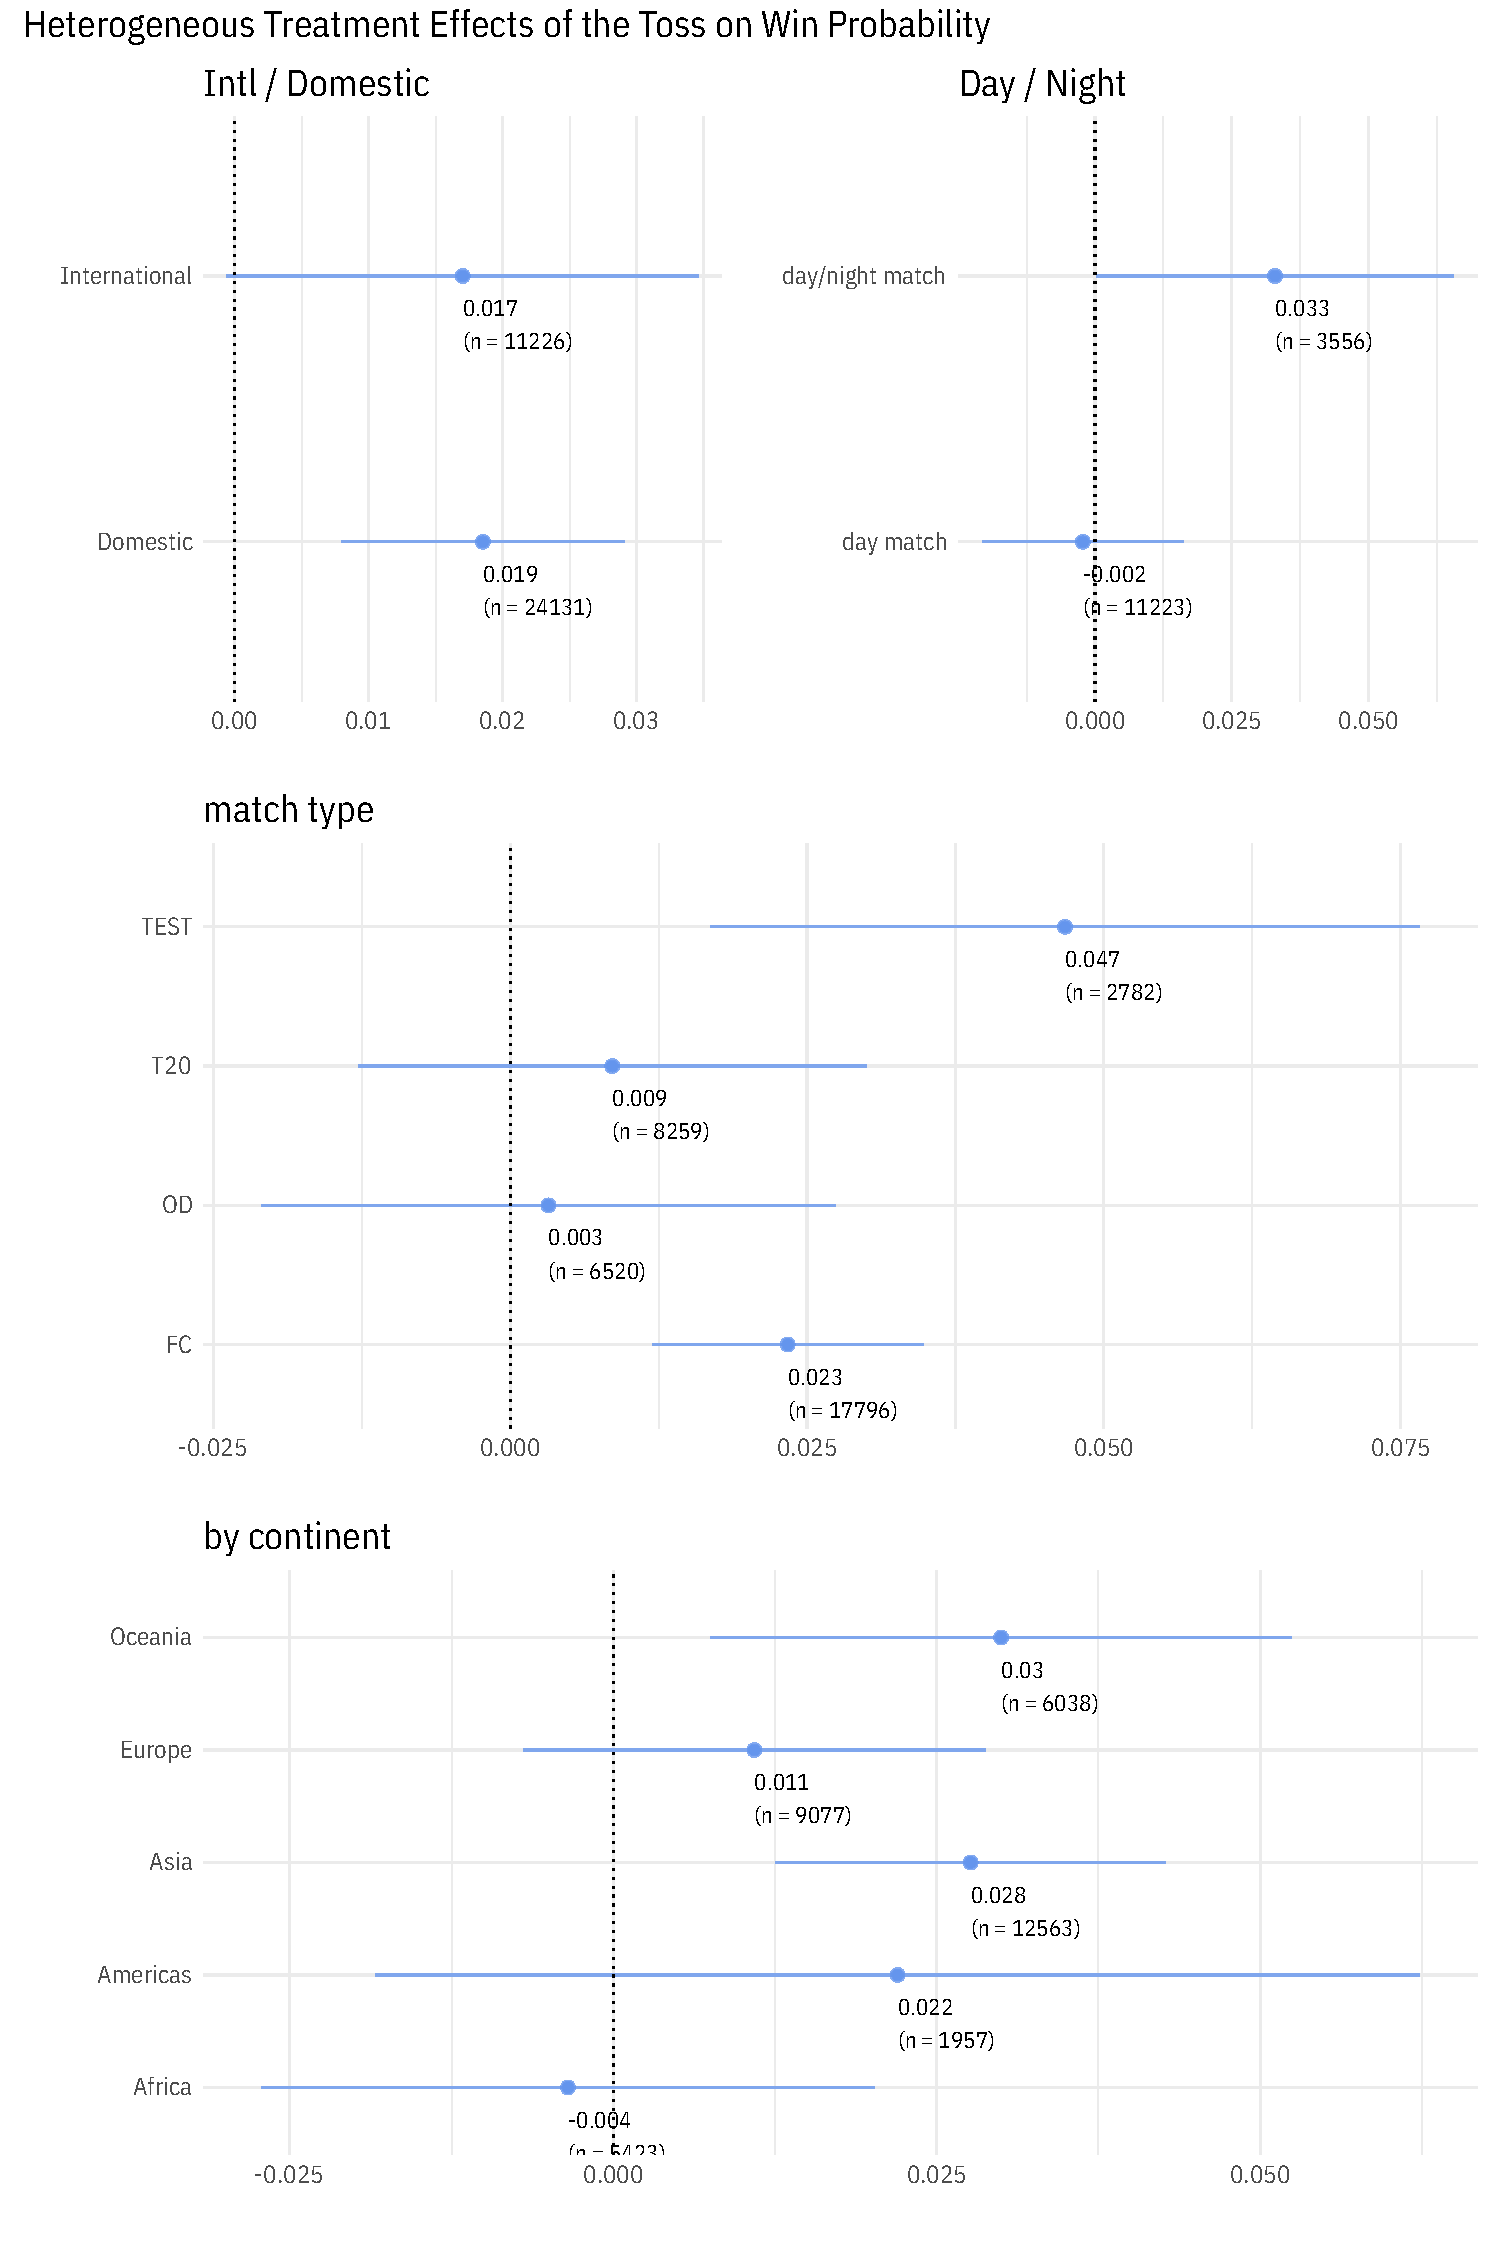
\includegraphics[scale=.5]{output/reduced_form_by_matchtype.pdf}
  \caption{The effect of winning the toss on win probability decomposed across different match types, over time, and by continent.}
  \label{fig:rf_het_TE}
\end{figure}

\clearpage

\begin{figure}[b]
  \centering
  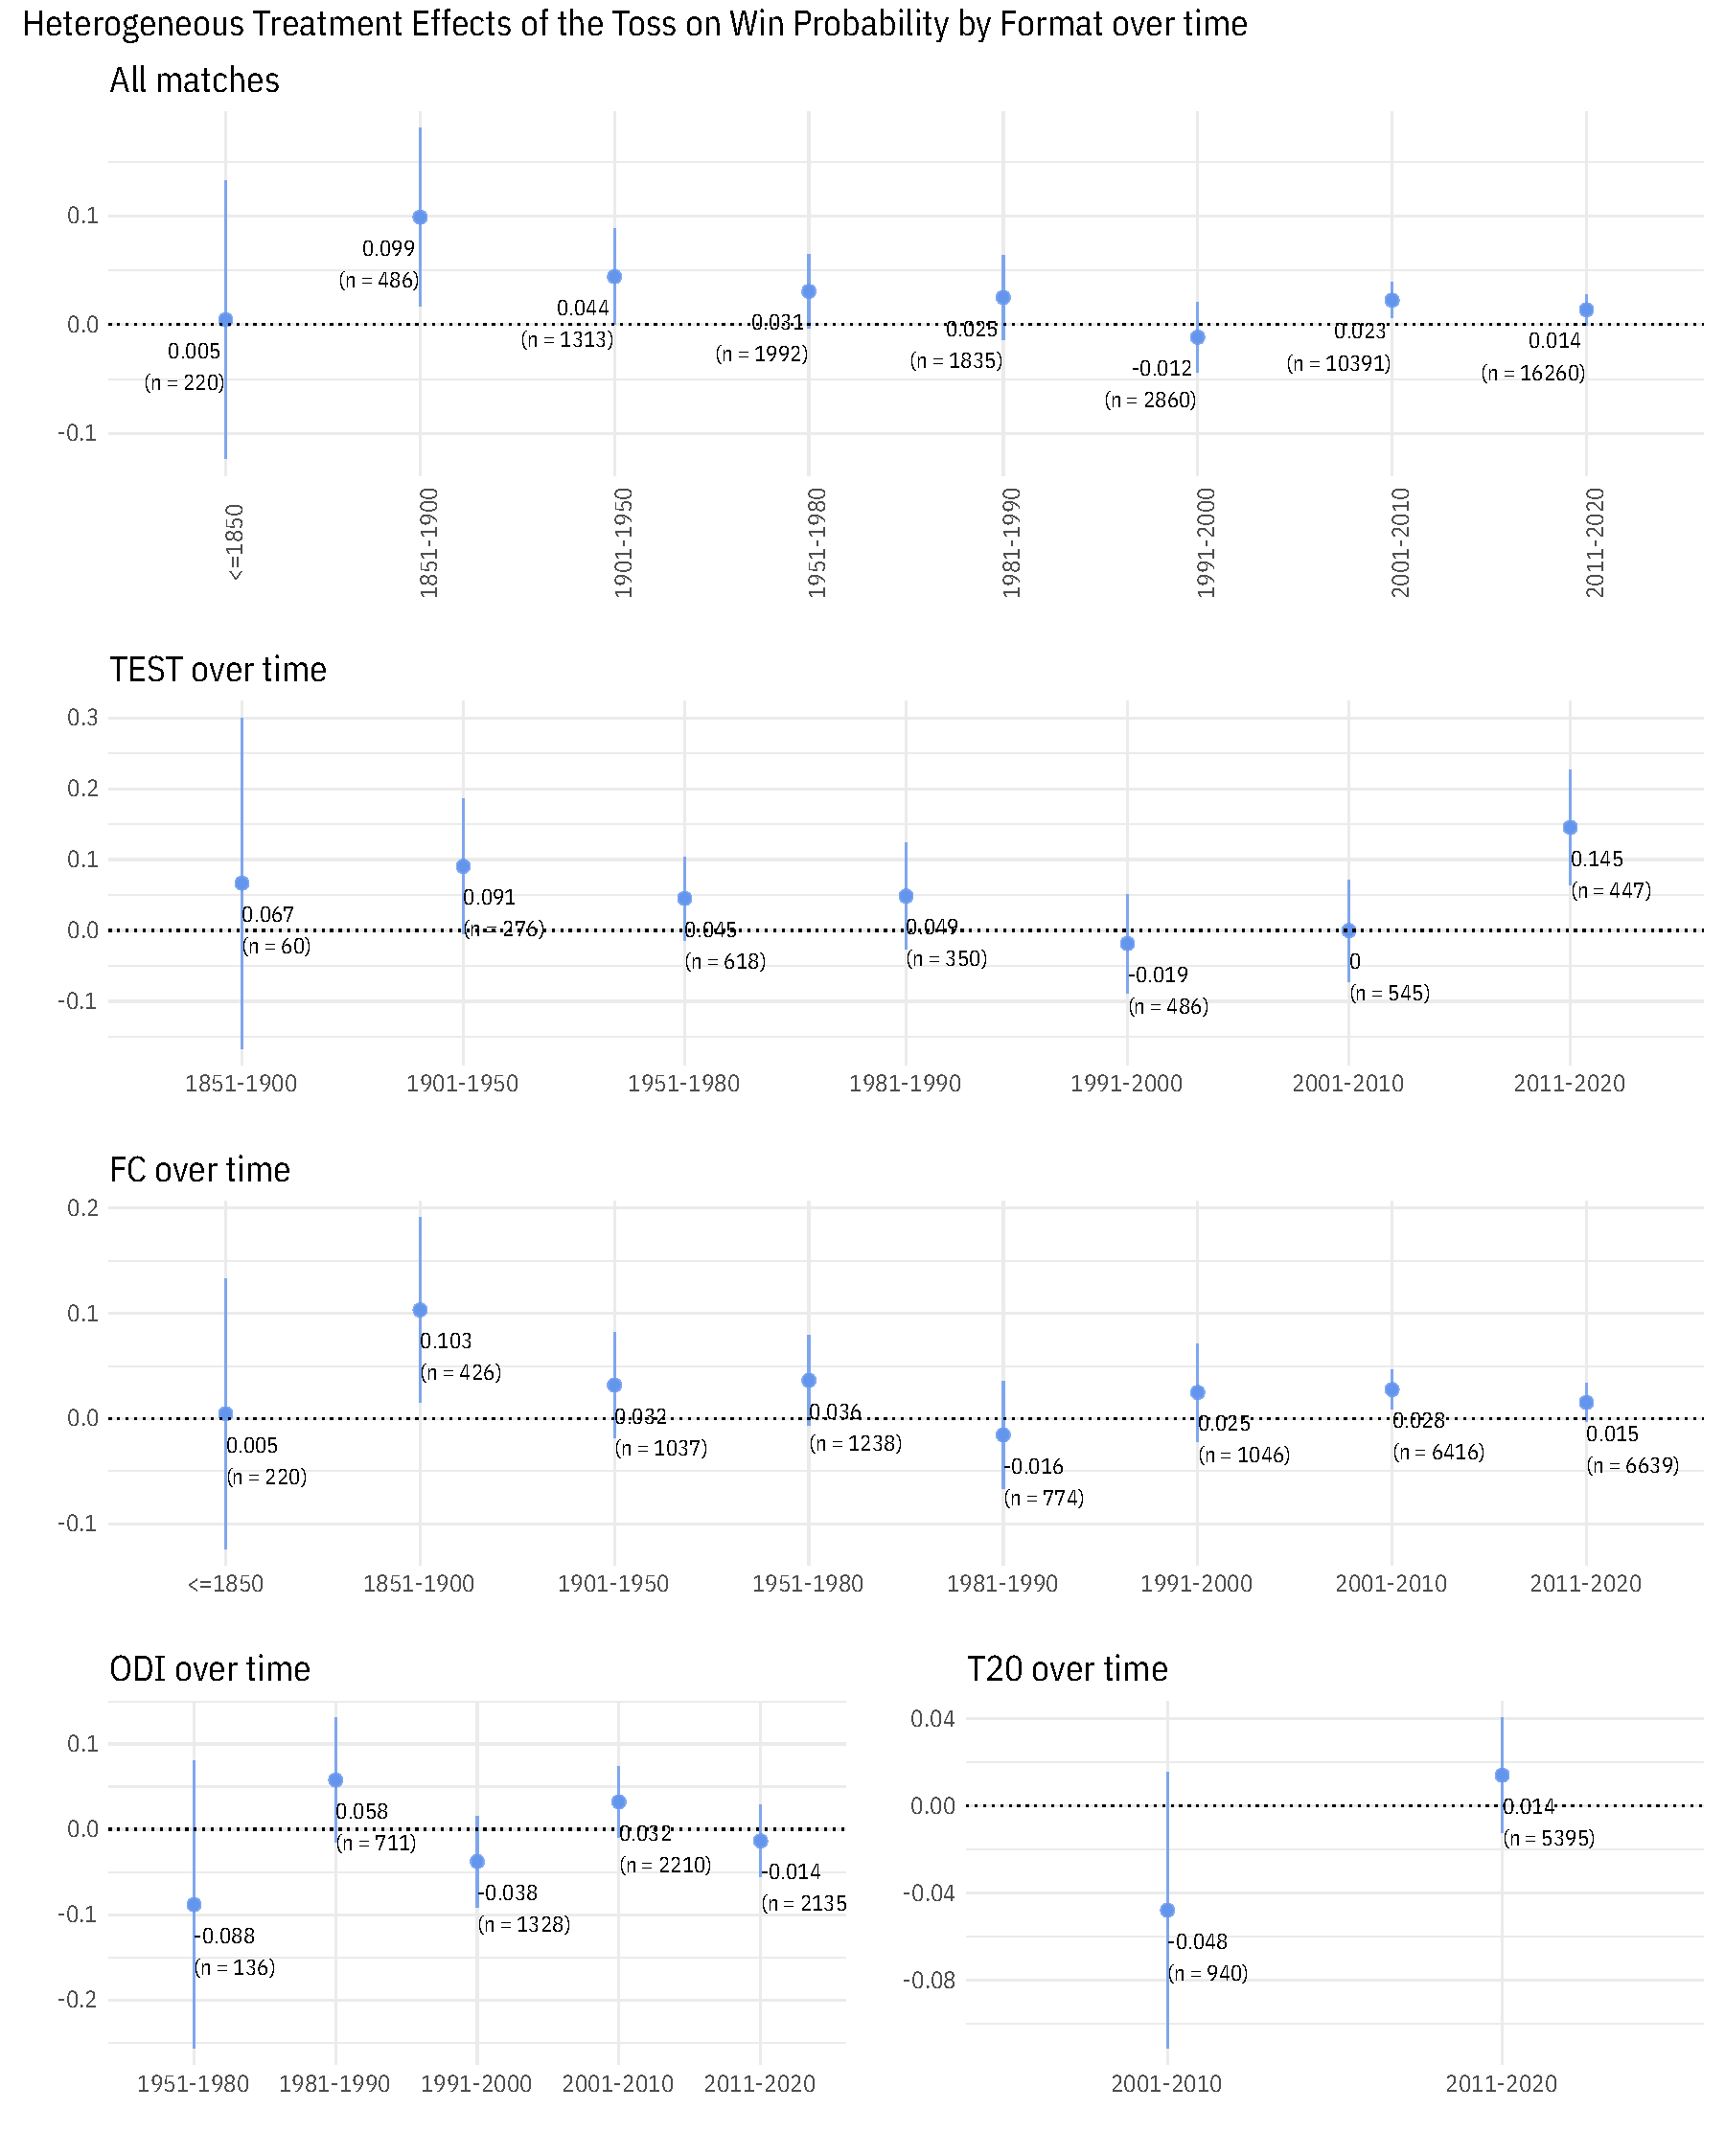
\includegraphics[scale=.5]{output/reduced_form_by_format_overtime.pdf}
  \caption{The effect of winning the toss on the probability of winning by format over time.}
  \label{fig:rf_het_TE2}
\end{figure}

\begin{figure}[b]
  \centering
  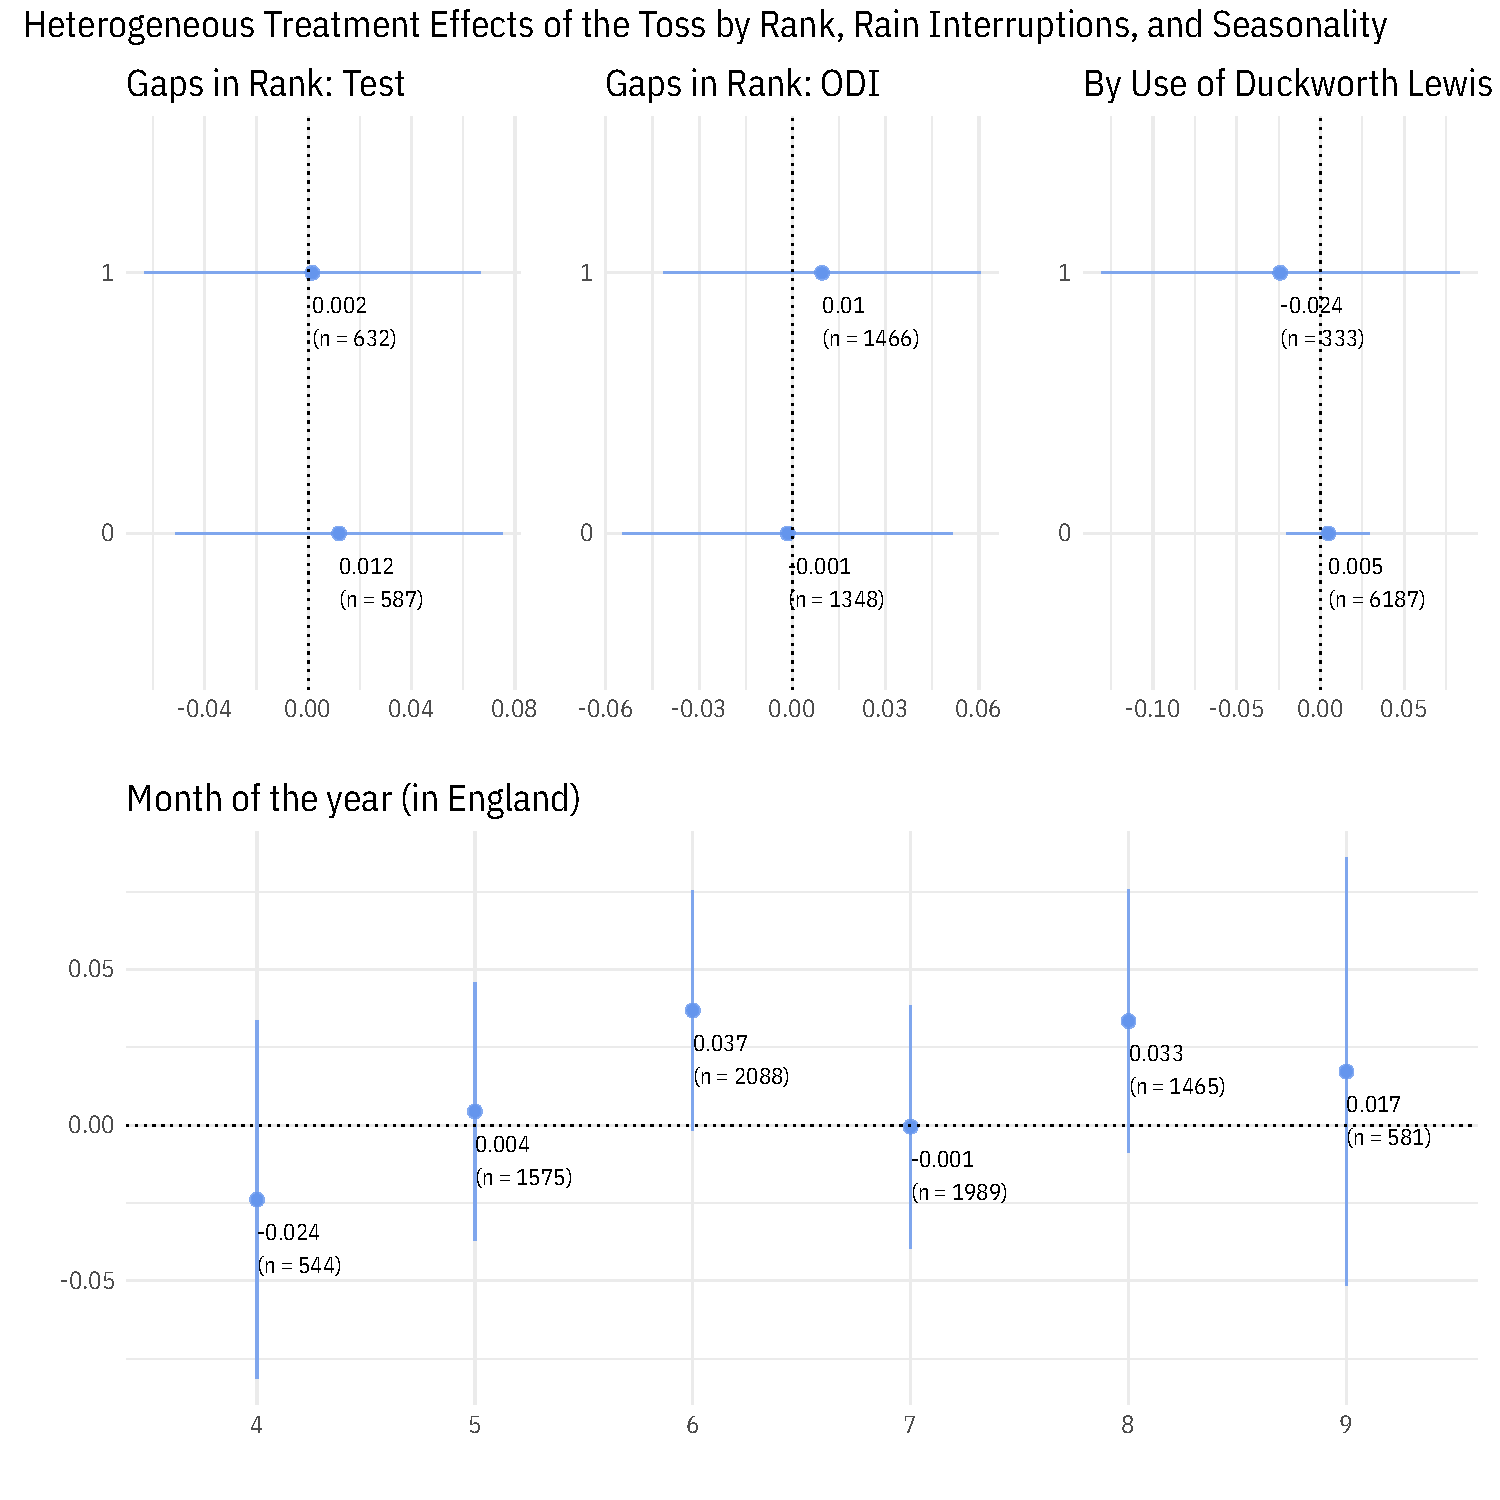
\includegraphics[scale=.5]{output/reduced_form_by_rank_dl_season.pdf}
  \caption{The effect of winning the toss on the probability of winning by competitiveness, use of DL, and seasonality.}
  \label{fig:rf_het_TE3}
\end{figure}

\clearpage

\begin{figure}
 \centering
 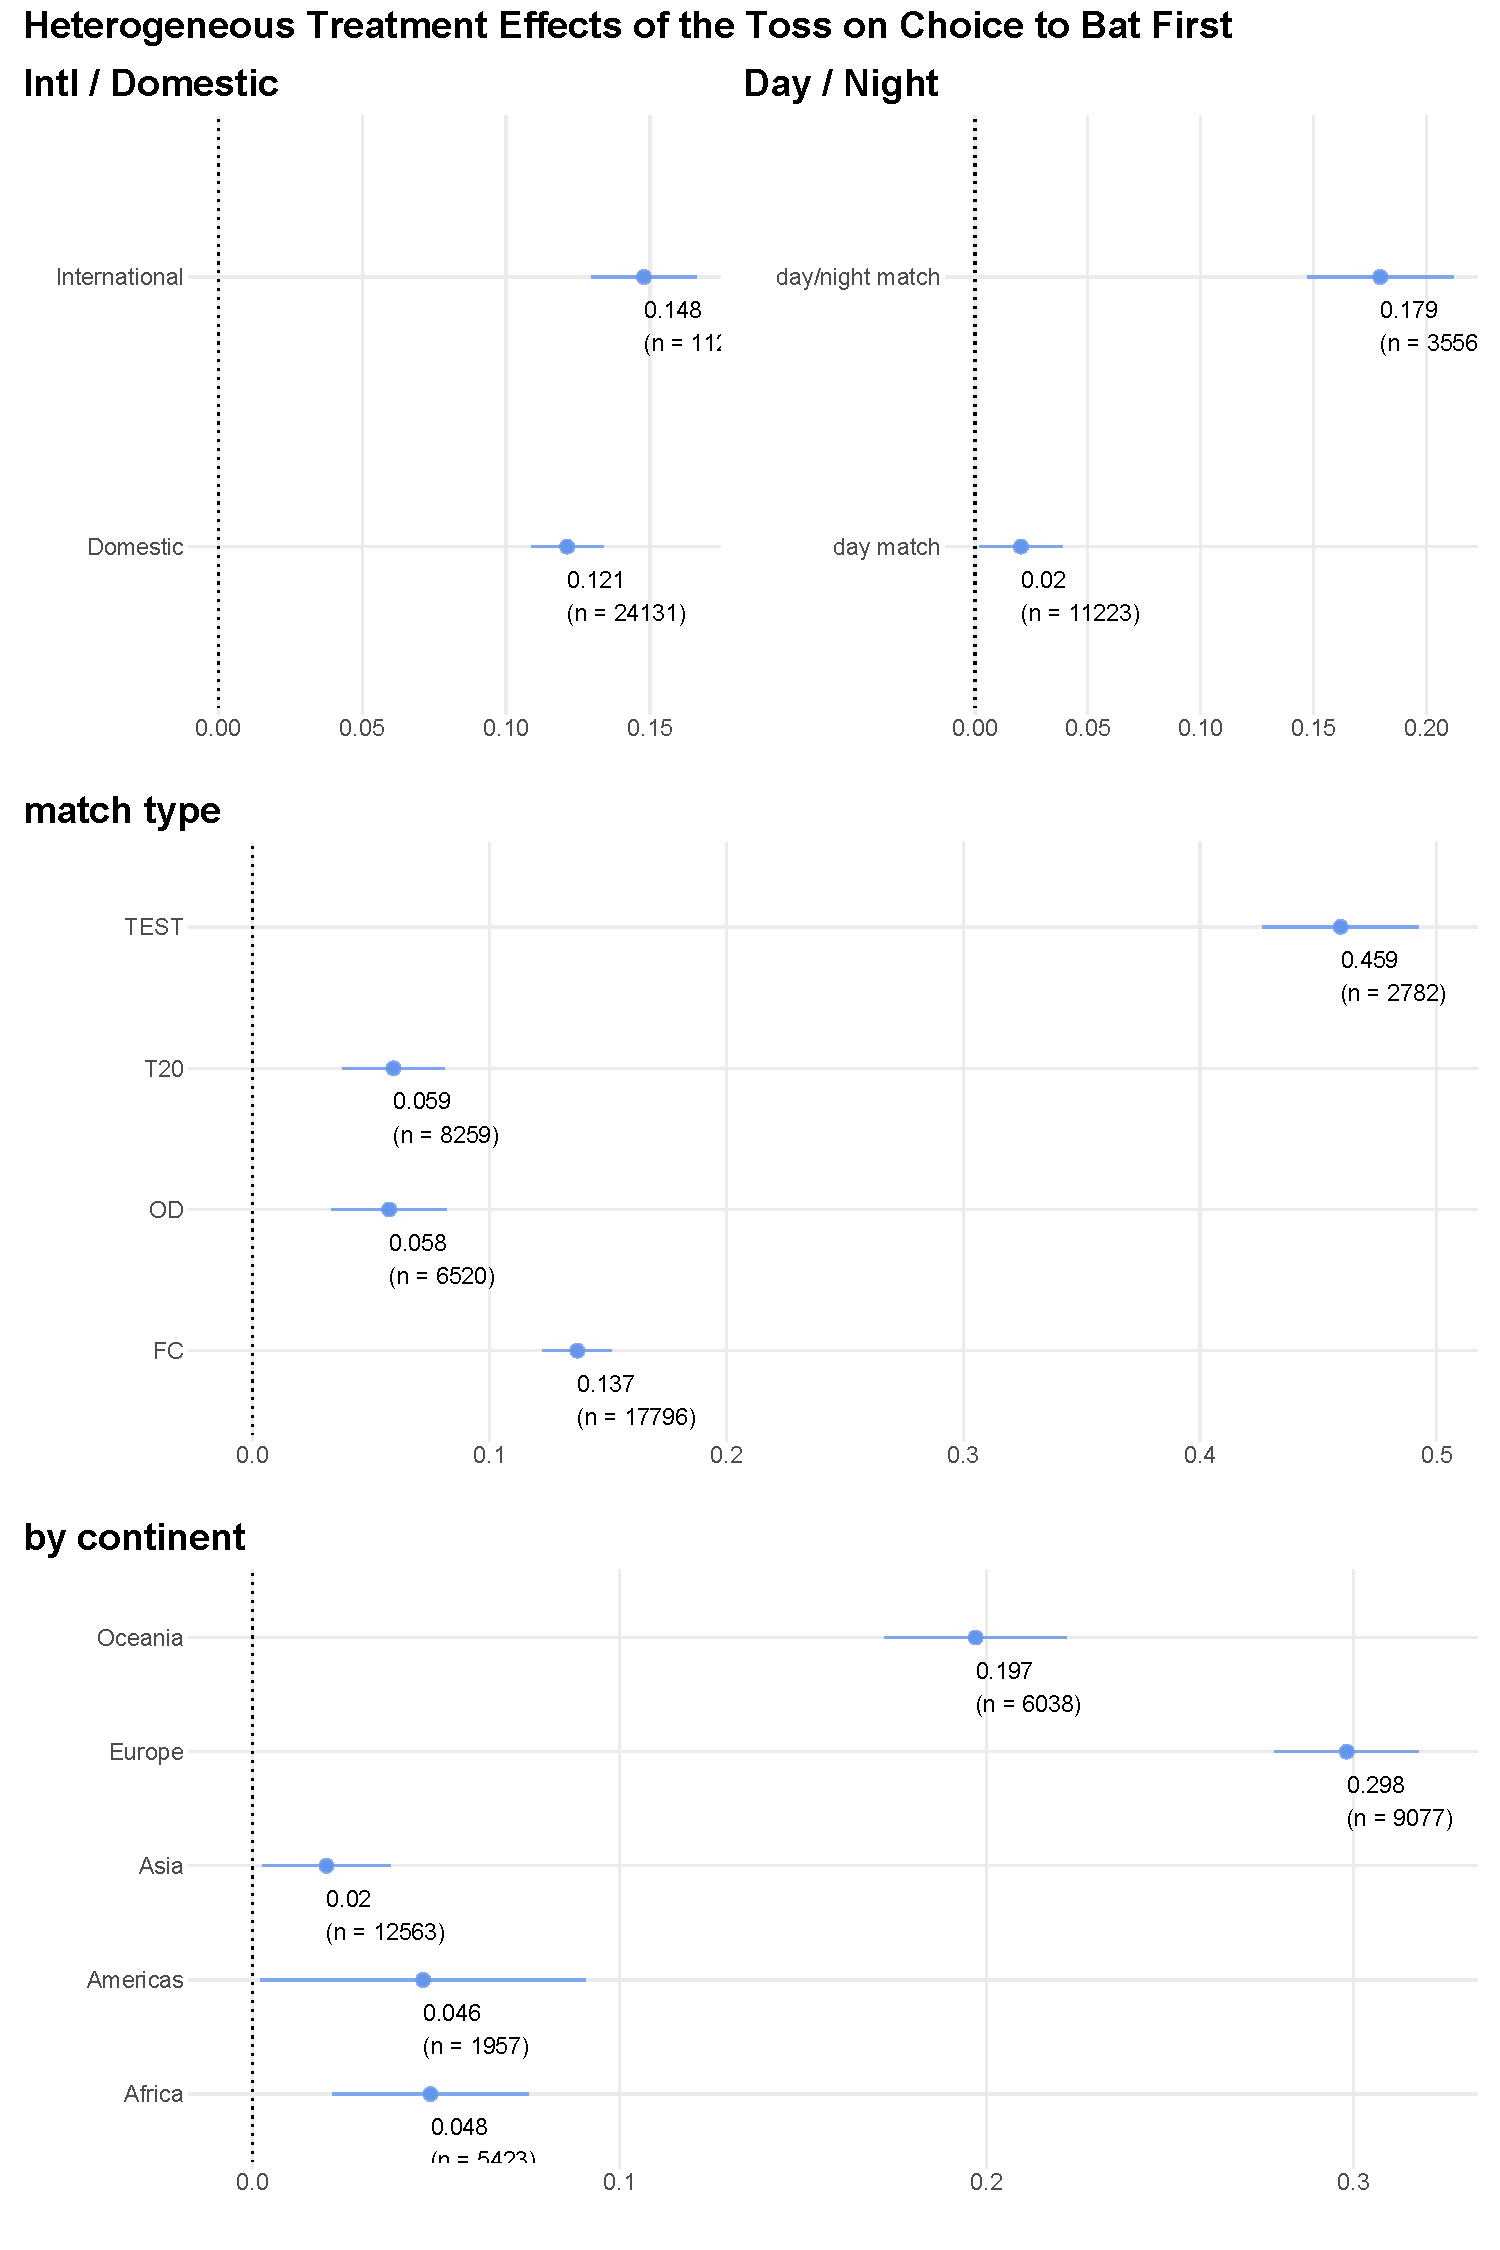
\includegraphics[scale=.5]{output/first_stage_by_matchtype.pdf}
 \caption{The effect of winning the toss on the choice to bat first across international and domestic matches, formats, and continents.}
 \label{fig:fs_het_TE1}
\end{figure}

\clearpage

\begin{figure}
 \centering
 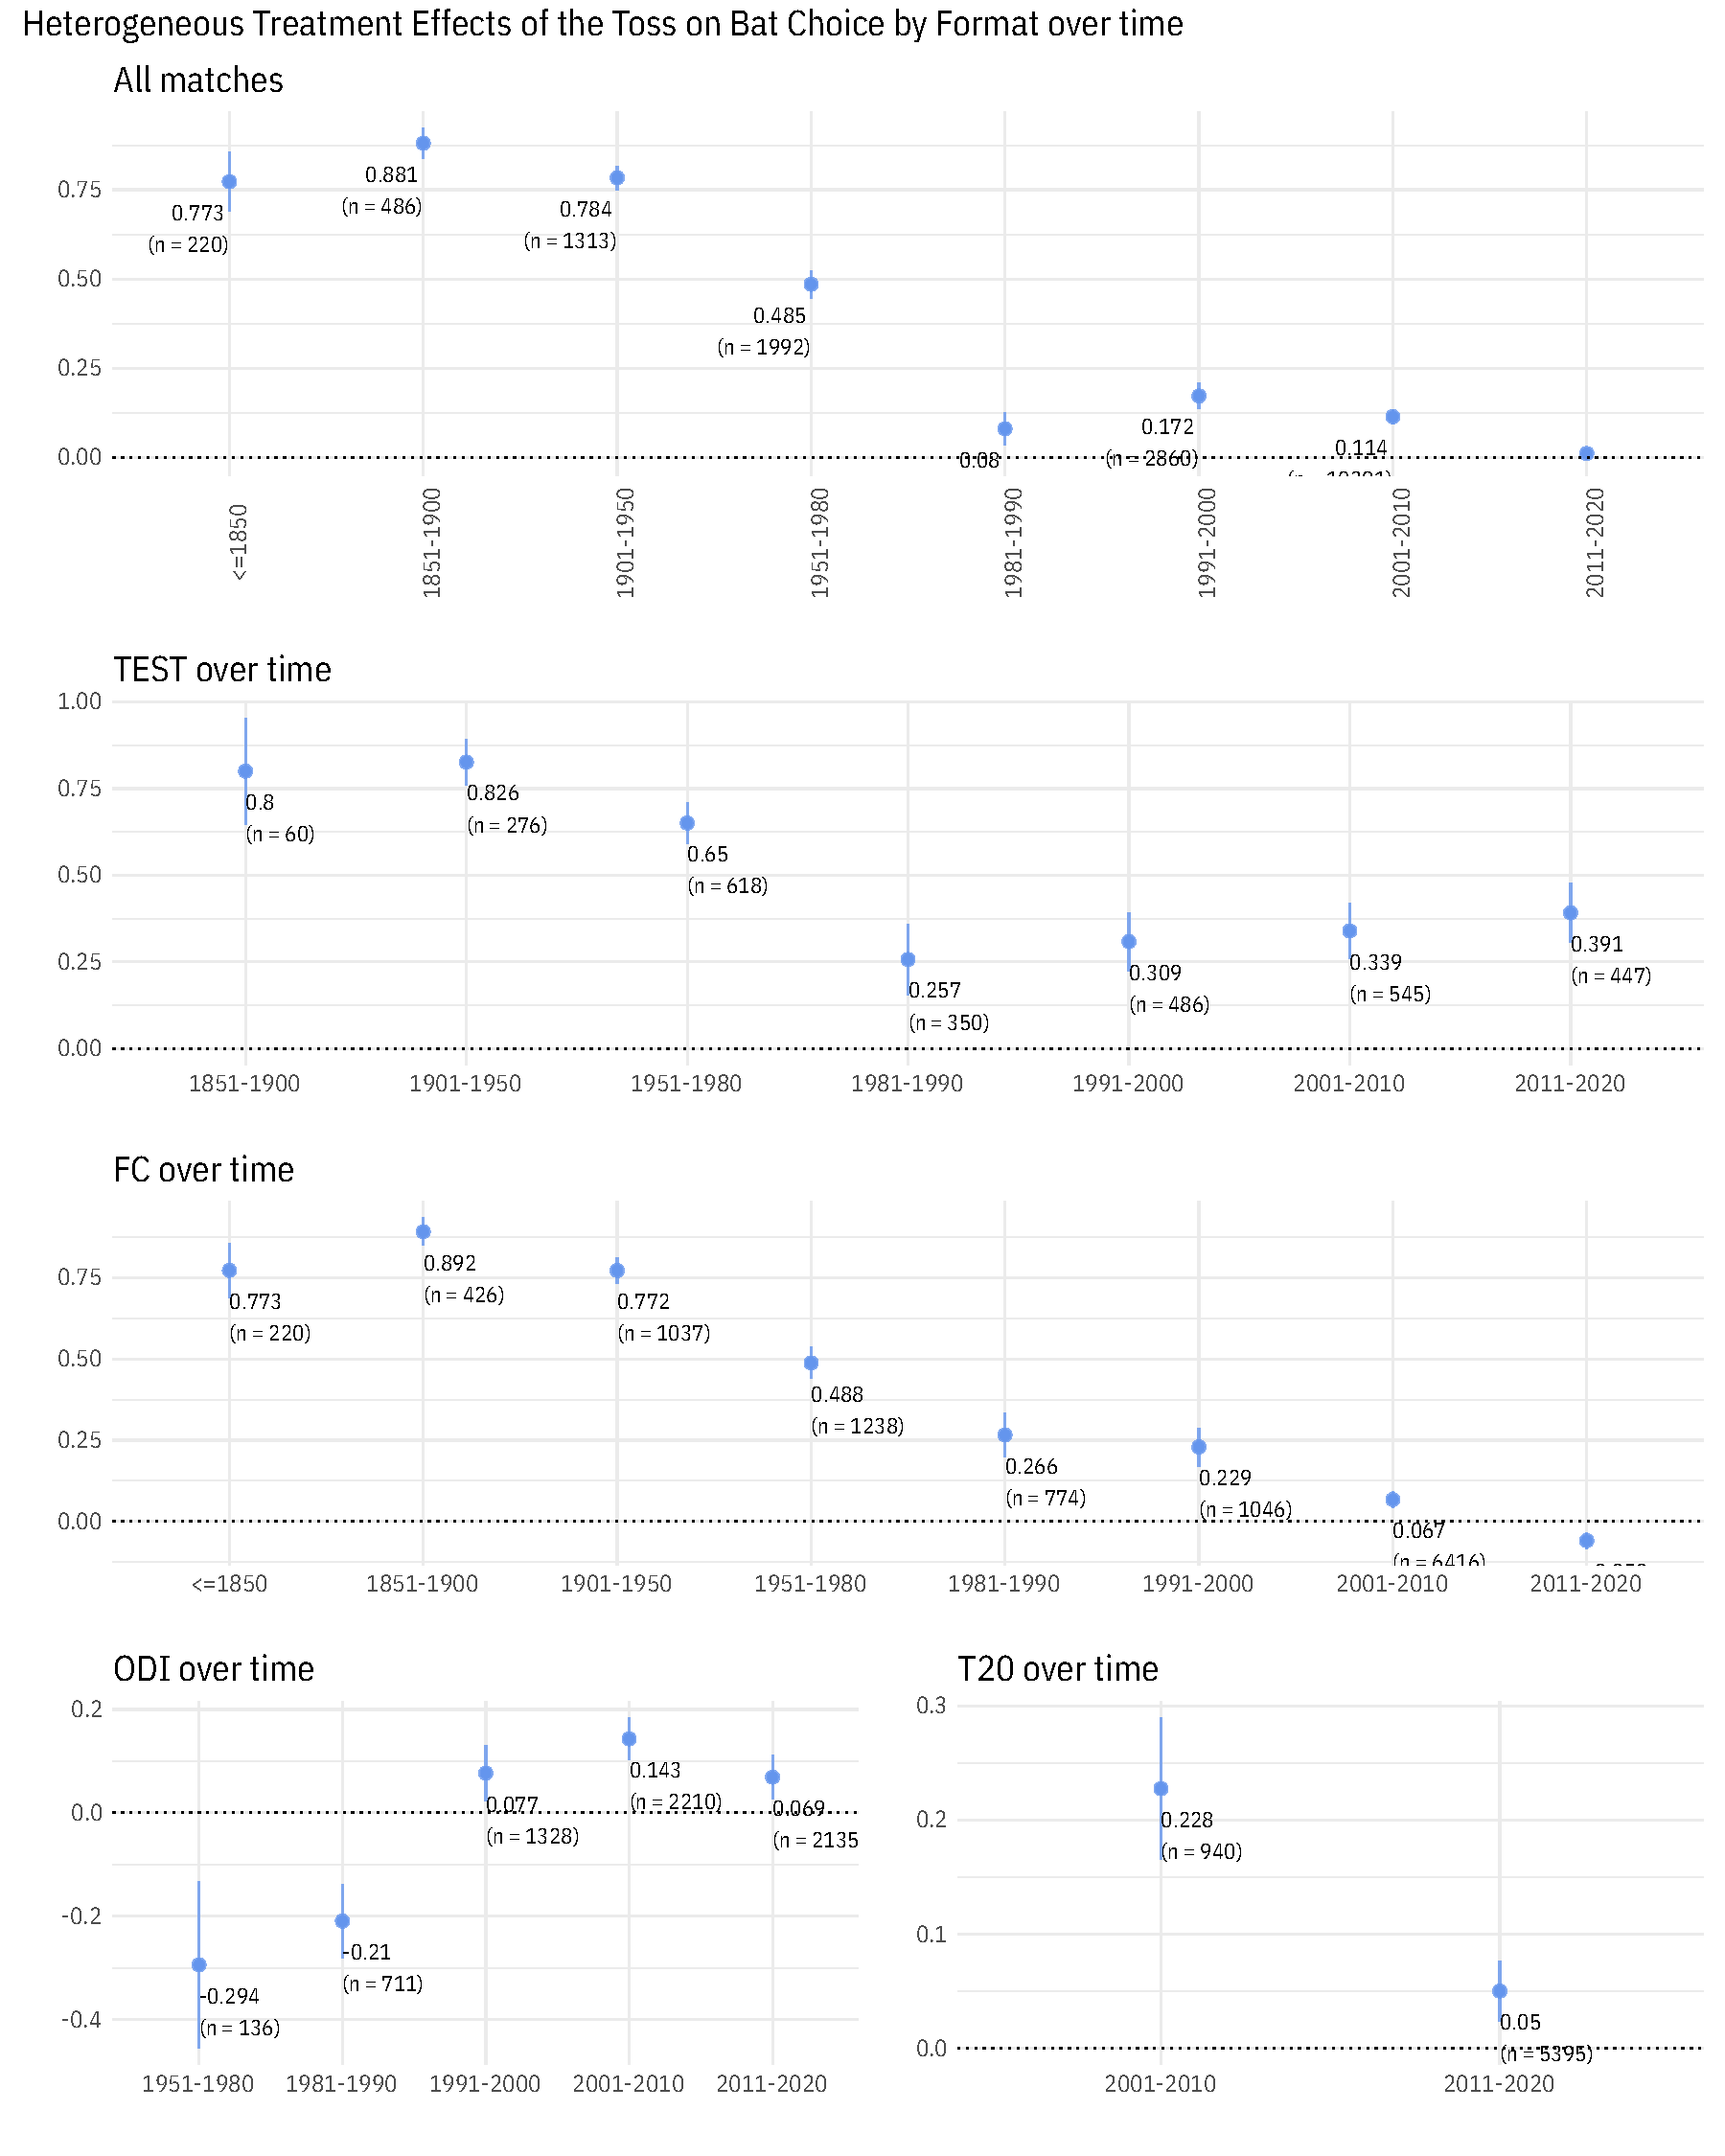
\includegraphics[scale=.5]{output/first_stage_by_format_overtime.pdf}
 \caption{The effect of winning the toss on the choice to bat first across different formats over time.}
 \label{fig:fs_het_TE2}
\end{figure}

\clearpage

\begin{figure}
 \centering
 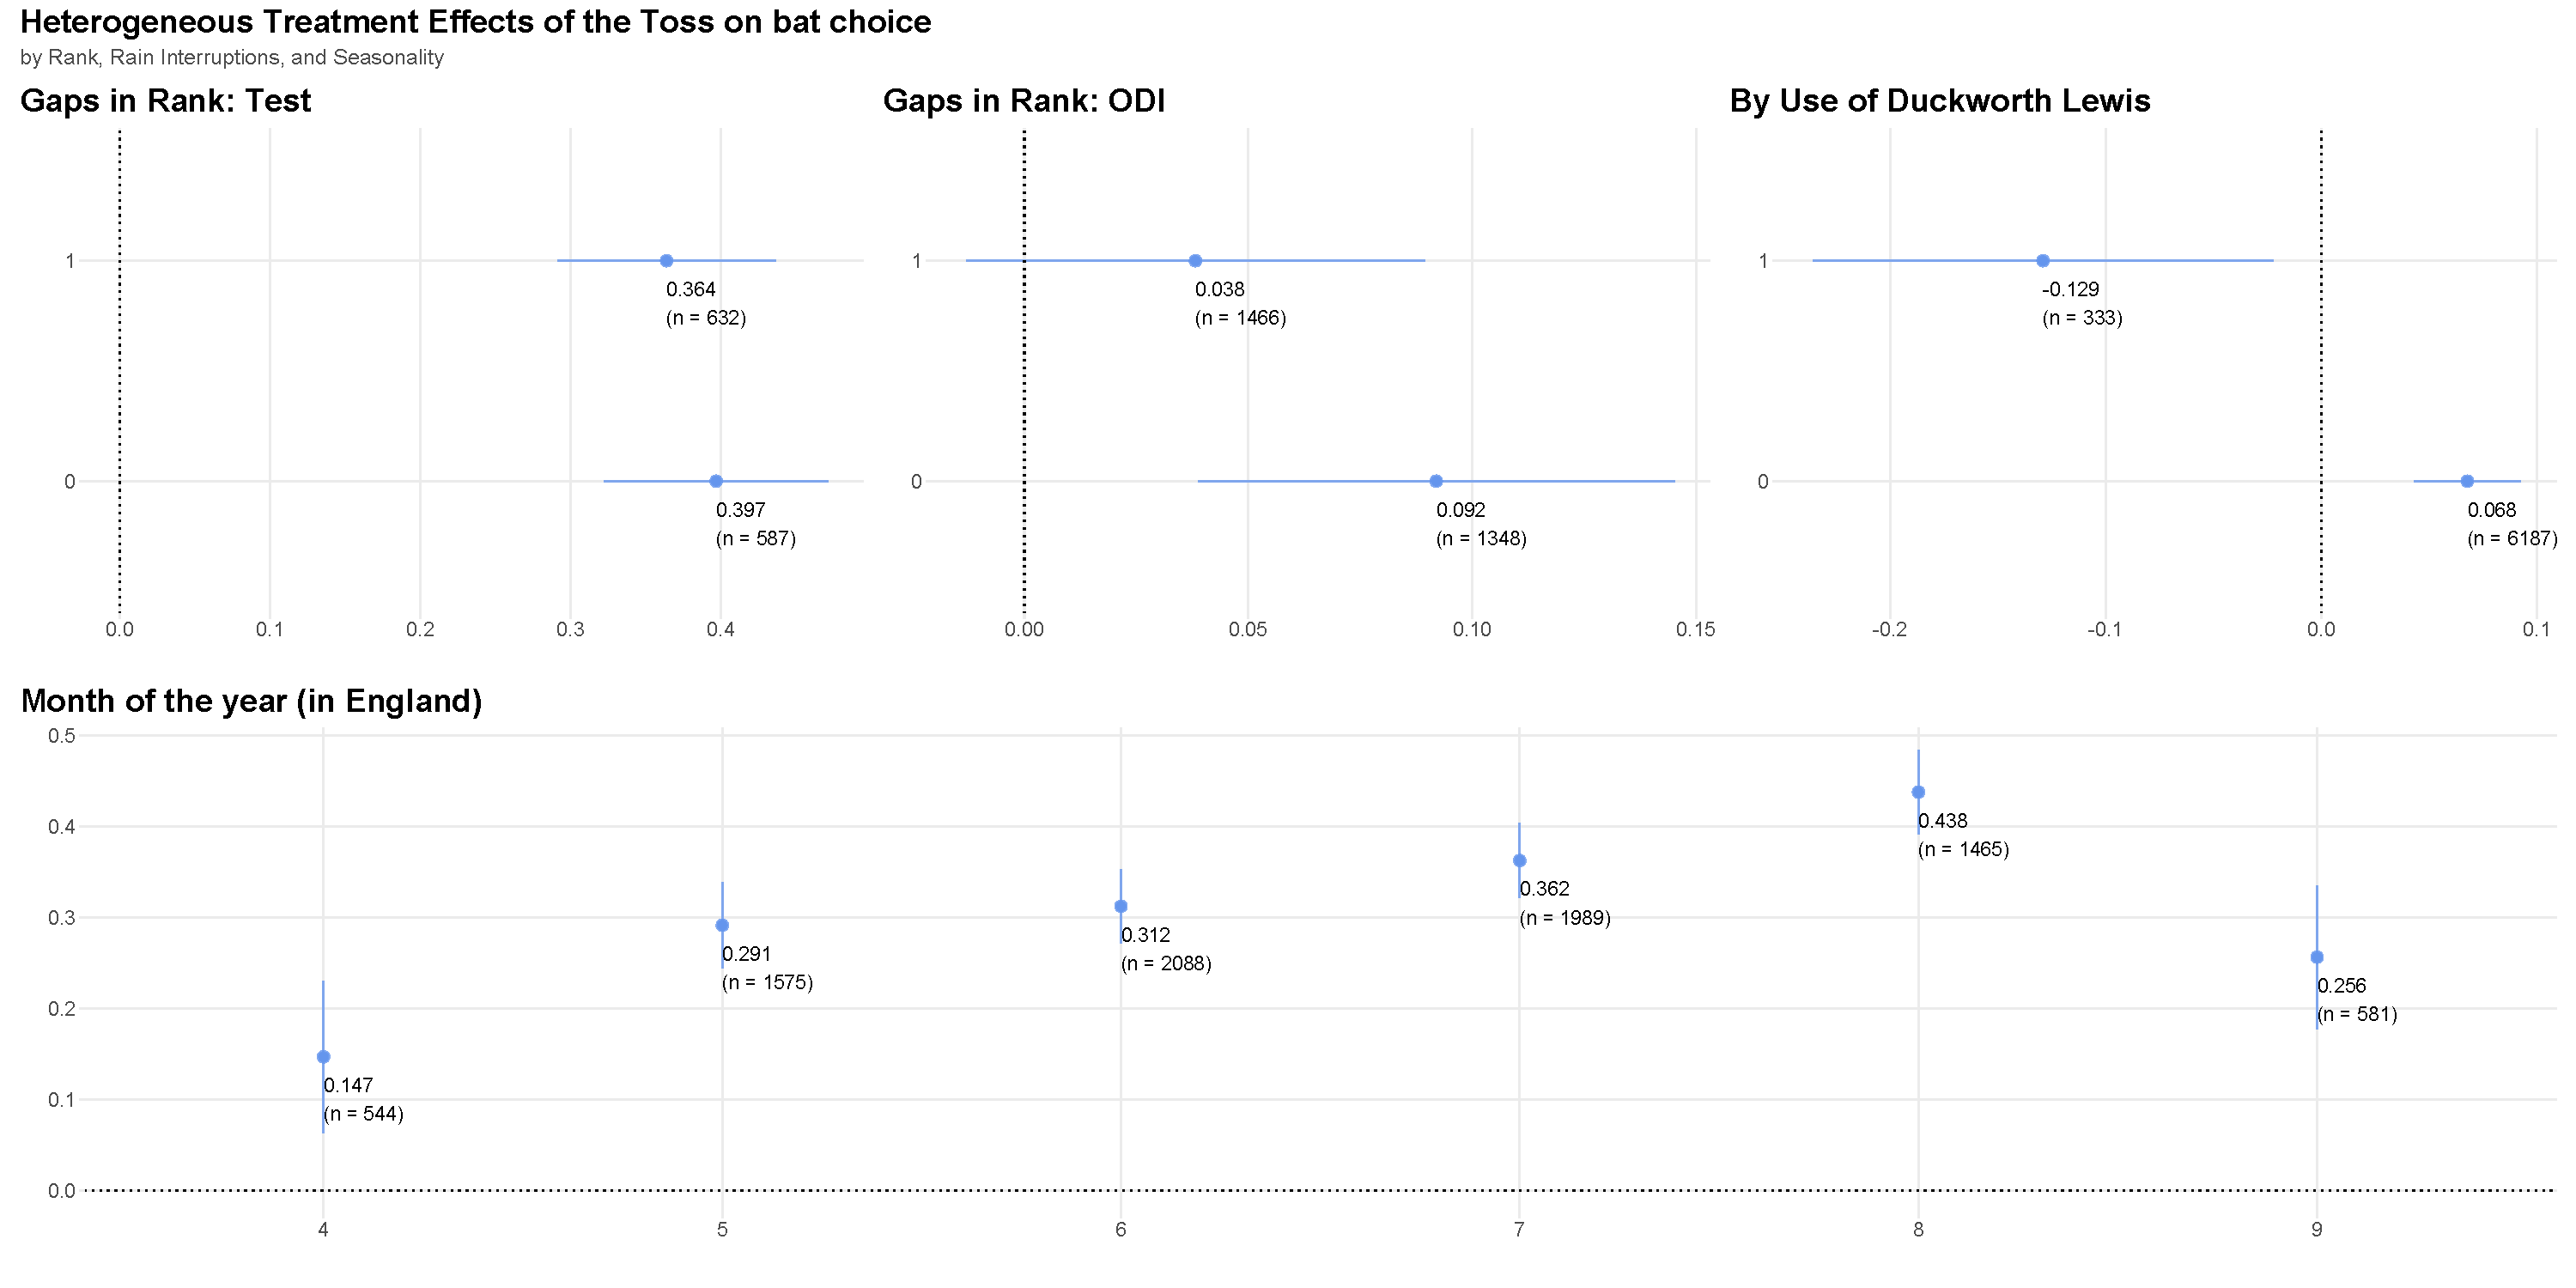
\includegraphics[scale=.5]{output/first_stage_by_rank_dl_season.pdf}
 \caption{The effect of winning the toss on the choice to bat first by rating differences, rain-interruptions, and season (in England)}
 \label{fig:fs_het_TE3}
\end{figure}



\end{document}
